\documentclass[12pt]{article}
\usepackage{color}
\usepackage{multicol,ifthen,booktabs,amsmath,amsfonts,bm,mathrsfs,amssymb}
\usepackage{times,mathptmx}
\usepackage{braket}
\usepackage{enumerate}
\usepackage{geometry}
\usepackage{graphicx}% Include figure files
\usepackage{listings}
\renewcommand\baselinestretch{1.5}\protect
\abovedisplayshortskip 3 pt
\belowdisplayshortskip 3 pt
\geometry{left=2cm,right=2cm,top=3cm,bottom=3cm}
\graphicspath{{./figures/}{./}}
\begin{document}

\section{Effective Action}
\begin{align}
\Gamma_k&=\int_x\bigg \{ \frac{1}{4} F_{\mu\nu}^a F_{\mu\nu}^a+Z_c (\partial_\mu \bar c^a) D_{\mu}^{a b} c^{b}+\frac{1}{2\xi}(\partial_\mu A_{\mu}^{a})^2\\ \nonumber
&+\frac{1}{2}\int_p A^a_{\mu}(-p) ({\Gamma_{AA}^{(2)}}_{\mu \nu}^{ab}-Z_A \Pi_{\mu \nu}^{\perp}\delta^{ab} p^2)A _{\nu}^b(p)\\  \nonumber
&+\bar q [Z_q (\gamma_\mu D_\mu-\gamma_0(\hat \mu+ig A_0)]q-\lambda_q \sum_{a=0}^8 [(\bar q T_a  q)^2+(\bar q i \gamma _5 T_a q)^2]\\  \nonumber
&+\bar q  h_{k}^{1/2}  \cdot \Sigma_{5} \cdot h_{k}^{1/2} q+tr \big (Z_{\Sigma,k}^{1/2} \cdot \partial_\mu\Sigma \cdot Z_{\Sigma,k}^{1/2}\cdot \partial_\mu\Sigma^\dagger\bigr) +\tilde U_k(\Sigma,\Sigma^\dagger)+V_{glue}(L,\bar L)
\bigg \}
\end{align}
here, the meson field :
\begin{align}
  \Sigma&=T^a(\sigma^a+i \pi^a)\,. \quad (a=0,1,...,8)\label{}
\end{align}
and 
\begin{align}
  \Sigma_5&=T^a(\sigma^a+i \gamma_5 \pi^a)\,. \quad (a=0,1,...,8)\label{}
\end{align}
with $T^a=\lambda^a/2(a=1,...,8)$ and $T^{0}=\frac{1}{\sqrt{2N_{f}}}\mathbb{I}_{N_{f}\times N_{f}}$ are generators of $SU(N_f=3)$. $\sigma^a$ and $\pi^a$ mean the scalar and pseudoscalar fields, respectively. The physical meson can be written obviously:
\begin{align}
\Sigma=\frac{1}{2}\begin{pmatrix}
a_0^0+\sigma_L+i\pi^0 + i\eta_L& \sqrt{2}(a_0^{+} +i \pi^{+}) & \sqrt{2} (\kappa^{+} +i K^{+})\\
\sqrt{2} (a_0^{-} +i \pi^{-}) & -a_0^0+\sigma_L - i\pi^0  + i\eta_L & \sqrt{2}(\kappa^0+i K^0) \\
\sqrt{2} (\kappa^{-} + i K^{-}) & \sqrt{2} (\bar \kappa^0 + i \bar K^0) & \sqrt{2} (\sigma_S + i \eta_S)\end{pmatrix}\label{eq:mesonmatrix}
\end{align}
the meson effective potential can be devided into three parts
\begin{align}
  \tilde{U}_{k}(\Sigma)&=U_k(\rho_1,\tilde{\rho}_2)-c_A \xi-c_L\sigma_L-c_S\sigma_S\,, \label{eq:tildeU}
\end{align}
here $U_k(\rho_1,\tilde{\rho}_2)$ is an arbitrary function of chiral symmetry invariant variables $\rho_1,\tilde{\rho}_2$.  $ c_A \xi$ is Kobayashi-Maskawa-’t Hooft trem which breaks $U_A(1)$ symmetry. The last two terms of Eq.(\ref{eq:tildeU}) are linear sigma terms, which break the chiral symmetry.
\begin{align}
  \rho_1&=\text{tr}(\Sigma \cdot \Sigma^\dagger)\,, \label{eq:rho1}\\[2ex]
  \tilde{\rho}_2&=\text{tr}\Big(\Sigma \cdot \Sigma^\dagger-\frac{1}{3}\,\rho_1\,\mathbb{I}_{3\times 3}\Big)^2 \,.\label{eq:rho2}
\end{align}
The Yukawa coupling 
\begin{align}
h_k=\begin{pmatrix} 
h_{l,k}&0&0\\
0&h_{l,k}&0\\
0&0&h_{s,k}
\end{pmatrix}
\end{align}
and meson and quark wave function renormalization
\begin{align}
Z_{\sigma,k}=\begin{pmatrix} 
Z_{\phi_l,k}&0&0\\
0&Z_{\phi_l,k}&0\\
0&0&Z_{\phi_s,k}
\end{pmatrix} 
\quad \quad
Z_{q,k}=\begin{pmatrix} 
Z_{l,k}&0&0\\
0&Z_{l,k}&0\\
0&0&Z_{s,k}
\end{pmatrix} 
\end{align}
At present, we assume $Z_{\sigma,k}=Z_{\pi,k}$ and $Z_{q,k}=Z_{l,k}$.

\section{Flow Equations}

The the Wetterich equation with dynamical hadronisation reads
\begin{align}
\partial_t \Gamma_k[\Phi]+\int \langle  \partial_t  \hat \phi_{k,i}\rangle \bigg ( \frac{\delta \Gamma_k [\Phi]}{\delta \phi_i}+j_\sigma \delta_{i \sigma}\bigg )
=\frac{1}{2} \text{Tr}(G_k[\Phi] \partial_t R_k)+\text{Tr}\bigg( G_{\phi \Phi_j} [\Phi] \frac{\delta \langle  \partial_t  \hat \phi_{k,i}\rangle}{\delta \Phi_j } R_{\phi} \bigg) \label{Wettericheq}
\end{align}
we assume 
\begin{align}
\langle  \partial_t  \hat \phi_{k}\rangle&= \dot{A}_{l,k}[(\bar q T_a  q)+(\bar q i \gamma _5 T_a q)]+\dot{A}_{s,k}[(\bar q T_b  q)+(\bar q i \gamma _5 T_b q)] +\dot{B}_k \Sigma,\\
&\text{for} \quad a=L,1,\cdot 3,b=4,\cdot7, S \nonumber
\end{align}
here $T^L,T^S$ are given in Appendix \ref{}
As pointed out in ref \cite{} , we choose $\dot{B}_k =0$.
By taking the derivative of of each side of Eq. (\ref{Wettericheq})
\begin{align}
\frac{\overrightarrow{\delta}}{\delta(\bar q T^a q)}(Eq. (\ref{Wettericheq}))\frac{\overleftarrow{\delta}}{\delta (\bar q T^a q)},
\end{align}
we get
\begin{align}
- \partial_t \lambda_q + \dot{A} h_{k}=-\text{Flow} _{(\bar q T^a q) (\bar q T^a q)}^{(4)}
\end{align}
with the condication
\begin{align}
\lambda_q  \equiv 0 , \quad \forall k
\end{align}
we get the renormalised hadronisation function
\begin{align}
\dot{\bar A}=-\frac{1}{\bar h_k}\overline{  \text{Flow} }_{(\bar q T^a q) (\bar q T^a q)}^{(4)}
\end{align}
we split the expression
\begin{align}
\dot{\bar A}_{l,k}=-\frac{1}{\bar h_{l,k}}\overline{  \text{Flow} }_{(\bar q T^L q) (\bar q T^L q)}^{(4)} \\
\dot{\bar A}_{s,k}=-\frac{1}{\bar h_{s,k}}\overline{  \text{Flow} }_{(\bar q T^S q) (\bar q T^S  q)}^{(4)}
\end{align}
And to calculate the yukawa flow equation:
\begin{align}
\frac{{\delta}}{\delta \sigma^a}\frac{{\delta}}{\delta(\bar q T^a q)}(Eq. (\ref{Wettericheq})) \quad a=L/S
\end{align}
we get
\begin{align}
\partial \bar h_{l,k}&=\bigg( \eta_{l,k} +\frac{1}{2}\eta_{\phi,k}\bigg )-\frac{\delta^2 \bar {\tilde U}(\Sigma)}{(\delta \bar \sigma_L)^2}\dot{\bar A}_{l,k}+\overline{  \text{Flow} }_{(\bar q T^L q) \sigma_L}^{(3)}\\
\partial \bar h_{s,k}&=\bigg( \eta_{s,k} +\frac{1}{2}\eta_{\phi,k}\bigg )-\frac{\delta^2 \bar {\tilde U}(\Sigma)}{(\delta \bar \sigma_S)^2}\dot{\bar A}_{s,k}+\overline{  \text{Flow} }_{(\bar q T^S q) \sigma_S}^{(3)}
\end{align}
A simpler way given in \cite{}
\begin{align}
\frac{{1}}{\sigma^a}\frac{{\delta}}{\delta(\bar q T^a q)}(Eq. (\ref{Wettericheq})) \quad a=L/S
\end{align}
and we get
\begin{align}
\partial \bar h_{l,k}&=\bigg( \eta_{l,k} +\frac{1}{2}\eta_{\phi,k}\bigg )-\frac{1}{\bar \sigma_L} \frac{\delta \bar{\tilde U}(\Sigma)}{\delta \bar \sigma_L}\dot{\bar A}_{l,k}+\frac{1}{\bar \sigma_L} \text{Re} \overline{  \text{Flow} }_{(\bar q T^L q)}^{(2)}\\
\partial \bar h_{s,k}&=\bigg( \eta_{s,k} +\frac{1}{2}\eta_{\phi,k}\bigg )-\frac{1}{\bar \sigma_S} \frac{\delta \bar{\tilde U}(\Sigma)}{\delta \bar \sigma_S}\dot{\bar A}_{s,k}+\frac{1}{\bar \sigma_S} \text{Re} \overline{  \text{Flow} }_{(\bar q T^S q)}^{(2)} \label{Yukawa_eq}
\end{align}
the next step is to calculate the $\overline{\text{Flow}}$ terms.

\section{Result}
Pressure:
\begin{align}
\frac{p}{T^4}=\frac{U(0,0)-U((T,\mu)}{T^4}
\end{align}
and  n-th order cumulats
\begin{align}
\chi^B_n=\frac{\partial^n}{\partial (\mu_B/T)^n}\frac{p}{T^4}
\end{align}
\begin{figure}[t]
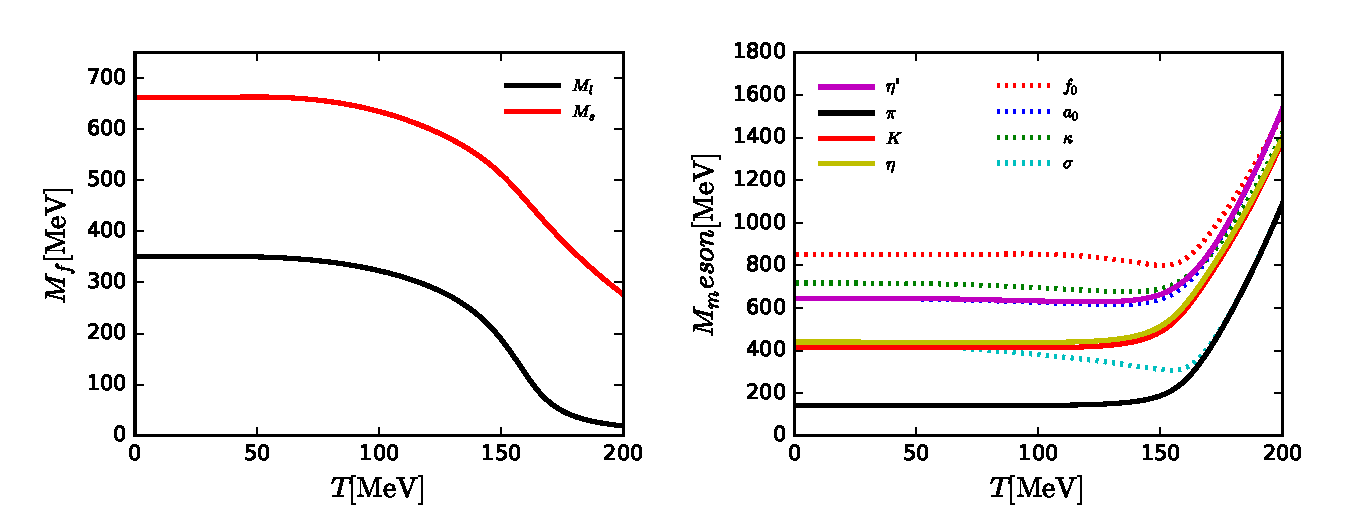
\includegraphics[width=1.\textwidth]{MFMBO}
\caption{Quark and meson masses as functions of temperature with js/jl=17.}
\end{figure}
\begin{figure}[t]
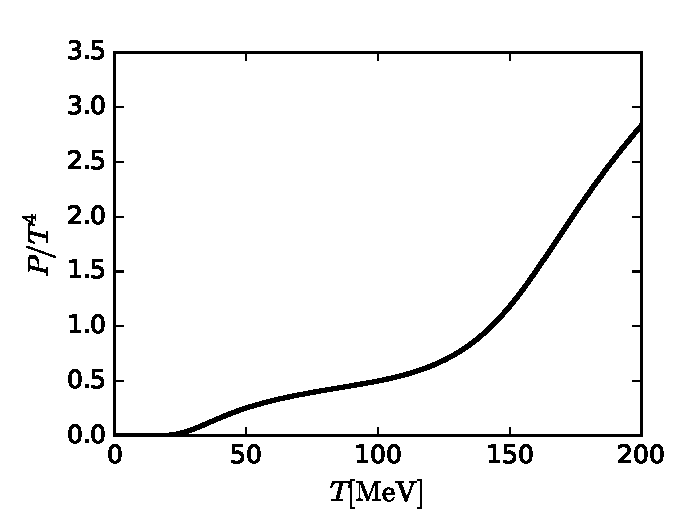
\includegraphics[width=0.5\textwidth]{PT4}
\caption{pressure}
\end{figure}
\begin{figure}[t]
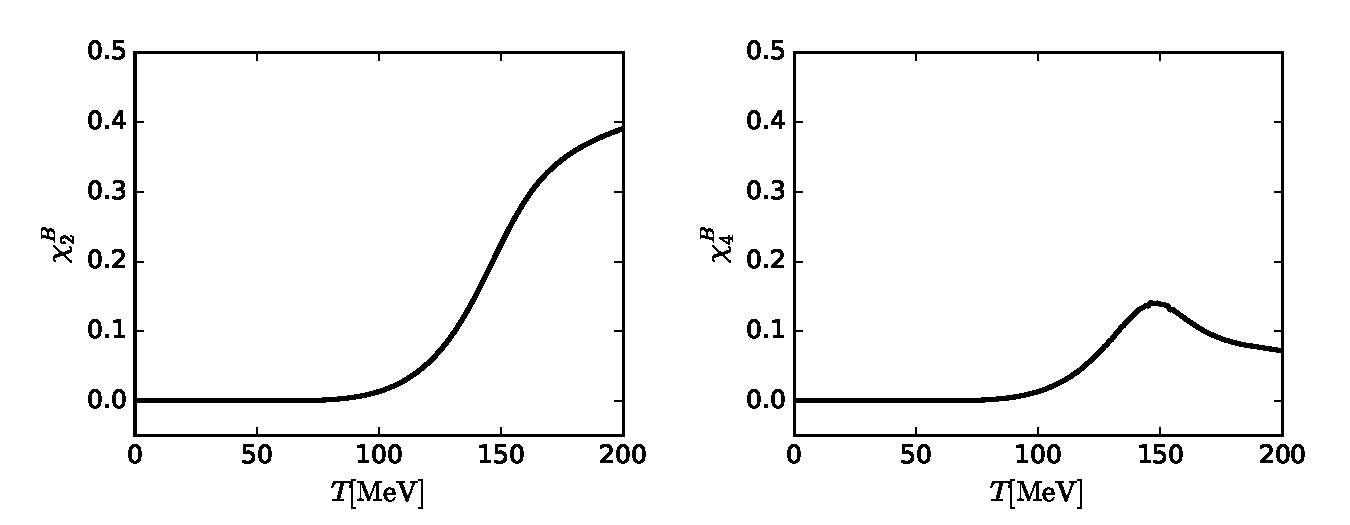
\includegraphics[width=1.\textwidth]{chi24}
\caption{cumulats,$T_{glue}=250MeV,\alpha=0.57$,}
\end{figure}
\begin{figure}[t]
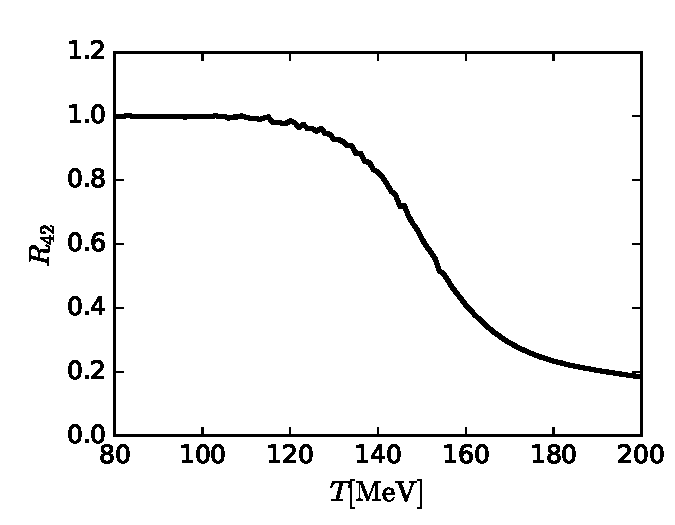
\includegraphics[width=0.5\textwidth]{R42}
\caption{ratio of cumulats}
\end{figure}
\begin{figure}[t]
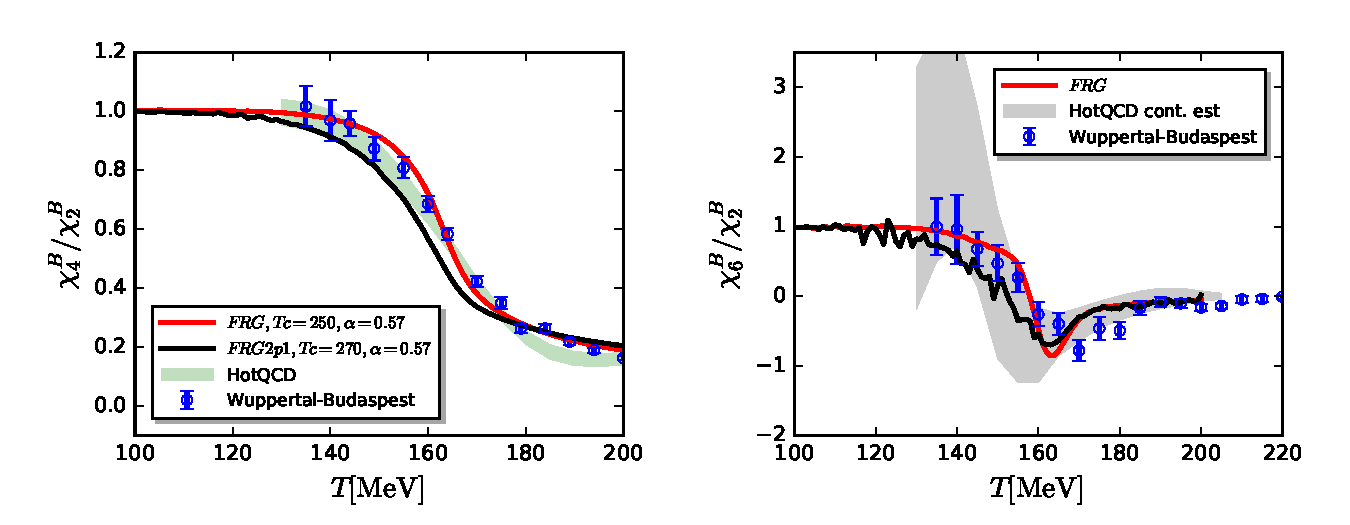
\includegraphics[width=1.\textwidth]{R42R62m}
\caption{ratio of cumulats}
\end{figure}
\section{Appendix.A}
The meson masses can be obtained by Hessian matrix:

\begin{align}
H_{p,LL}=&\frac{c_A \sigma_S}{\sqrt{2}}+\frac{1}{6} U^{(0,1)} (\sigma_L^2-2 \sigma_S^2)+U^{(1,0)}\\
H_{p,LS}=&\frac{c_A \sigma_L}{\sqrt{2}}\\
H_{p,SS}=&U^{(1,0)} - \frac{1}{3} U^{(0,1)} (\sigma_L^2 - 2 \sigma_S^2)\\
H_{p,11}=&-\frac{c_A \sigma_S}{\sqrt{2}}+\frac{1}{6} U^{(0,1)} (\sigma _L^2-2\sigma_S^2)+U^{(1,0)}\\
H_{p,44}=&- \frac{c_A \sigma_L}{2} + U^{(1,0)} +
 \frac{1}{6} U^{(0,1)}(\sigma_L^2- 3 \sqrt{2} \sigma_L \sigma_S+4 \sigma_S^2)
\end{align}
\begin{align}
H_{s,LL}=&-\frac{c_A \sigma_S}{\sqrt{2}}+U^{(1,0)}+U^{(2,0)} \sigma_L^2 + \frac{1}{6} U^{(0,1)} (3 \sigma_L^2-2 \sigma_S^2)\\ \nonumber
&+\frac{1}{36} \sigma_L^2 (\sigma_L^2-2 \sigma_S^2)(U^{(0,2)} (\sigma_L^2-2\sigma_S^2)+12 U^{(1,1)})\\
H_{s,LS}=&-\frac{c_A \sigma_L}{\sqrt{2}}+U^{(2,0)} \sigma_L \sigma_S-\frac{2}{3} U^{(0,1)} \sigma_L \sigma_S \\ \nonumber
&-\frac{1}{18} U^{(0,2)} \sigma_L \sigma_S (\sigma_L^2-2 \sigma_S^2)^2-\frac{1}{6} U^{(1,1)}\sigma_L \sigma_S (\sigma_L^2-2 \sigma_S^2)\\
H_{s,SS}=&U^{(1,0)}+U^{(2,0)}\sigma_S^2 - \frac{1}{3} U^{(0,1)} (\sigma_L^2 - 6 \sigma_S^2) \\ \nonumber
&+\frac{1}{9} \sigma_S^2 (- 6 U^{(1,1)} (\sigma_L^2 - 2 \sigma_S^2) +
    U^{(0,2)} (\sigma_L^2 - 2 \sigma_S^2)^2)\\
H_{s,11}=&\frac{c_A \sigma_S}{\sqrt{2}}+U^{(1,0)} + \frac{1}{6} U^{(0,1)}(7 \sigma_L^2 - 2 \sigma_S^2)\\
H_{s,44}=&\frac{c_A \sigma_L}{2}+U^{(1,0)}+\frac{1}{6} U^{(0,1)} (\sigma_L^2+3 \sqrt{2} \sigma_L\sigma_S+4 \sigma_S^2)
\end{align}

The coefficients in Eq.(\ref{Yukawa_eq} are given as
\begin{align}
\frac{1}{\sigma_L} \frac{\delta \tilde U(\Sigma)}{\delta \sigma_L}&=
U^{(1,0)} - \frac{c_A \sigma_S}{\sqrt{2}} + \frac{1}{6}U^{(0,1)} (\sigma_L^2 - 2 \sigma_S^2)\\
\frac{1}{\sigma_S} \frac{\delta \tilde U(\Sigma)}{\delta \sigma_L}&=
U^{(1,0)}- \frac{ck \sigma_L^2}{2 \sqrt{2} \sigma_S} - \frac{1}{3} U^{(0,1)} (\sigma_L^2 - 2 \sigma_S^2)
\end{align}
One interesting thing is that  $\frac{1}{\sigma_L} \frac{\delta \tilde U(\Sigma)}{\delta \sigma_L}=m_\pi^2$.

the three-point meson vertex are defined as
\begin{align}
\lambda_{\phi_i,\phi_j,\phi_l,k}=\frac{\partial^3 U_k(\Sigma)}{\partial \phi_i,\partial \phi_j,\partial \phi_l}\bigg |_{\phi_0}
\end{align}
because we assume
\begin{align}
Z_\phi=Z_{\pi^+}
\end{align}
we choose the three-point meson vertex involve one $\pi^+$, which are given as
\begin{align}
\lambda_{\pi^+\pi^-f_0,k}&=\frac{1}{36}\{18 \sqrt{2} c_A \sin \phi_S  \\ \nonumber
&+ 2 \sin\phi_S \sigma_S [12 U^{(0,1)} - 18 U^{(2,0)}+ (\sigma_L^2 - 2 \sigma_S^2) (3 U^{(1,1)} +  U^{(0,2)} \sigma_L^2 - 2 U^{(0,2)} \sigma_S^2)] \\ \nonumber
& +\cos\phi_S \sigma_L [12 U^{(0,1)} +  36 U^{(2,0)} + (\sigma_L^2 - 2 \sigma_S^2) (12 U^{(1,1)} +  U^{(0,2)} \sigma_L^2 - 2 U^{(0,2)} \sigma_S^2)]\}
\end{align}
\begin{align}
\lambda_{\pi^+\pi^-\sigma,k}&=\frac{1}{36}\{-18 \sqrt{2} c_A \cos\phi_S\\ \nonumber
&- 2 \cos\phi_S \sigma_S [12 U^{(0,1)} -  18 U^{(2,0)} + (\sigma_L^2 - 2 \sigma_S^2) (3 U^{(1,1)} + U^{(0,2)} \sigma_L^2 - 2 U^{(0,2)} \sigma_S^2)] \\ \nonumber
&+ \sin\phi_S \sigma_L [12 U^{(0,1)} + 36 U^{(2,0)} + (\sigma_L^2 - 2 \sigma_S^2) (12 U^{(1,1)} + U^{(0,2)} \sigma_L^2 - 2 U^{(0,2)} \sigma_S^2)]\}
\end{align}
\begin{align}
\lambda_{\pi^+a_0^-\eta,k}&=\sin\phi_P \frac{c_A} {\sqrt{2}} + \cos\phi_P U^{(0,1)} \sigma_L\\
\lambda_{\pi^+a_0^-\eta',k}&=-\cos\phi_P\frac{ck}{\sqrt{2}} + \sin\phi_P U^{(0,1)} \sigma_L\\
\lambda_{\pi^+\kappa^-K^0,k}&=\lambda_{\pi^+K^-\kappa^0,k}=\frac{c_A}{\sqrt{2}} + U^{(0,1)} \sigma_S
\end{align}
\section{Appendix.B}

As we defined
\begin{equation}
\begin{split}
\rho_1&=\frac{1}{2}(\sigma_l^2+\sigma_s^2)\\
\rho_2&=\frac{1}{24}(\sigma_l^2-2 \sigma_s^2)^2
\end{split}
\end{equation}
Note that
\begin{equation}
\sigma_l < \sqrt{2} \sigma_s
\end{equation}
then
\begin{equation}
\begin{split}
2 \rho_1 & = \sigma_l^2 + \sigma_s^2 \\
-2 \sqrt{6 \rho_2} &=\sigma_l^2-2 \sigma_s^2
\end{split}
\end{equation}
then
\begin{equation}
\begin{split}
\sigma_l^2 &= \frac{2}{3}(2\rho_1-\sqrt{6 \rho_2})\\
\sigma_s^2 &= \frac{2}{3} ( \rho_1 + \sqrt{6 \rho_2})
\end{split}
\end{equation}
so
\begin{equation}
\begin{split}
\frac{\partial\sigma_l^2}{\partial \rho_1} &= \frac{4}{3} \quad
\frac{\partial\sigma_l^2}{\partial \rho_2} = -\frac{\sqrt{6}}{3} \rho_2^{-1/2} \\
\frac{\partial\sigma_s^2}{\partial \rho_1} &= \frac{2}{3} \quad
\frac{\partial\sigma_s^2}{\partial \rho_2} = \frac{\sqrt{6}}{3} \rho_2^{-1/2}
\end{split}
\end{equation}
so we get
\begin{equation}
\frac{\partial\sigma_l^2}{\partial \rho_2}=
-\frac{\partial\sigma_s^2}{\partial \rho_2}
\end{equation}
and
\begin{equation}
\frac{\partial^2 \sigma_l^2}{\partial \rho_2^2}=
- \frac{\partial^2 \sigma_s^2}{\partial \rho_2^2}=
\frac{\sqrt{6}}{6}\rho_2^{-3/2}
\end{equation}
The quark masses are given as
\begin{equation}
m_l^2=h^2 \frac{\sigma_l^2}{4} \quad m_s^2 =h^2 \frac {\sigma_s^2}{2}
\end{equation}
therefore
\begin{equation}
\begin{split}
\frac{\partial m_l^2}{\partial \rho_2} &
= -\frac{1}{2} \frac{\partial m_s^2}{\partial \rho_2}
= -\frac{\sqrt{6}}{12}h^2\rho_2^{-1/2}\\
\frac{\partial^2 m_l^2}{\partial \rho_2^2} &
=-\frac{1}{2}\frac{\partial^2 m_s^2}{\partial \rho_2^2}
=\frac{\sqrt{6}}{24}h^2 \rho_2^{-3/2}
\end{split}
\end{equation}
The quark loop function
\begin{equation}
l^{(f)}=\frac{1}{3}\Big(1-\frac{\eta_q}{4}\Big)\frac{1}{\sqrt{1+\bar m _f^2}}(1-n_f(E+\mu)-n_f(E-\mu))
\end{equation}
here $\bar m_f$ is dimensionless mass.

Then the light and strange quarks part of the the potential flow:
\begin{equation}
\partial_t U= -4 N_c \frac{k^4}{4\pi^2} \Big[2l^{(f)}(\bar m_l^2)+l^{(f)}(\bar m_s^2)\Big]
\end{equation}
For simplify,we only consider the square brackets above:
\begin{equation}
A_{qk}= 2l^{(f)}(\bar m_l^2)+l^{(f)}(\bar m_s^2)
\end{equation}
and
\begin{equation}
\begin{split}
\frac{\partial A_{qk}}{\partial \rho_2}
&=2 \frac{\partial l^{(f)}(\bar m_l^2)}{\partial \bar m_l^2} \frac{\partial \bar m_l^2}{\partial \rho_2}
+\frac{\partial l^{(f)}(\bar m_s^2)}{\partial \bar m_s^2} \frac{\partial \bar m_s^2}{\partial \rho_2}\\
&=2 \frac{\partial \bar m_l^2}{\partial \rho_2} \Big(\frac{\partial l^{(f)}(\bar m_l^2)}{\partial \bar m_l^2} - \frac{\partial l^{(f)}(\bar m_s^2)}{\partial \bar m_s^2}\Big)
\end{split}
\end{equation}

We consider $T=0$ case:
\begin{equation}
l^{(f)}=\frac{1}{3}\Big(1-\frac{\eta_q}{4}\Big)\frac{1}{\sqrt{1+\bar m _f^2}}
\end{equation}
then
\begin{equation}
\begin{split}
\frac{\partial A_{qk}}{\partial \rho_2}
&=2 \frac{\partial \bar m_l^2}{\partial \rho_2} \Big(\frac{\partial l^{(f)}(\bar m_l^2)}{\partial \bar m_l^2} - \frac{\partial l^{(f)}(\bar m_s^2)}{\partial \bar m_s^2}\Big)\\
&=- \frac{\partial \bar m_l^2}{\partial \rho_2} \frac{1}{3}\Big(1-\frac{\eta_q}{4}\Big)\Big((1+\bar m_l^2)^{-3/2}-(1+ \bar m_s^2)^{-3/2}\Big)
\end{split}
\end{equation}
Because $\bar m_q^2 \ll 1,\bar m_l^2 \sim 5\times 10^{-16}$ at $k=\Lambda$, we use Taylor expansion
\begin{equation}
\begin{split}
\frac{\partial A_{qk}}{\partial \rho_2}
&=- \frac{1}{3} \Big(1-\frac{\eta_q}{4} \Big) \frac{\partial \bar m_l^2}{\partial \rho_2}
 \Big((1-\frac{3}{2} \bar m_l^2 +\frac{15}{8} \bar m_l^4 \cdots)-(1-\frac{3}{2} \bar m_s^2 + \frac{15}{8} \bar m_s^4+\cdots)\Big)\\
&=- \frac{1}{3} \Big(1-\frac{\eta_q}{4} \Big) \Big( -\frac{\sqrt{6}}{12} \frac{h^2}{k^2}\rho_2^{-1/2}\Big)
 \Big(-\frac{3}{2} (\bar m_l^2 - \bar m_s^2) +\frac{15}{8} (\bar m_l^4 - \bar m_s^4 )+\cdots\Big)\\
 &=-\frac{\sqrt{6}}{24}\Big(1-\frac{\eta_q}{4} \Big) \Big( \frac{h^2}{k^2}\rho_2^{-1/2}\Big)
 \Big((\bar m_l^2 - \bar m_s^2) -\frac{5}{4} (\bar m_l^4 - \bar m_s^4 )+\frac{35}{24} (\bar m_l^6 - \bar m_s^6)\cdots\Big)
 \end{split}
\end{equation}

If we consider second order derivative, it will be worse:
\begin{equation}
\begin{split}
\frac{\partial}{\partial \rho_2}\Big(\frac{\partial A_{qk}}{\partial \rho_2}\Big)
&= 2 \Big[\frac{\partial^2 \bar m_l^2}{\partial \rho_2^2}\Big(\frac{\partial l^{(f)}(\bar m_l^2)}{\partial \bar m_l^2} - \frac{\partial l^{(f)}(\bar m_s^2)}{\partial \bar m_s^2}\Big)
+ \frac{\partial \bar m_l^2}{\partial \rho_2} \Big(\frac{\partial \bar m_l^2}{\partial \rho_2} \frac{\partial^2 l^{(f)}(\bar m_l^2)}{\partial (\bar m_l^2)^2} - \frac{\partial \bar m_s^2}{\partial \rho_2} \frac{\partial^2 l^{(f)}(\bar m_s^2)}{\partial (\bar m_s^2)^2 }\Big) \Big]\\
&= 2 \Big[\frac{\partial^2 \bar m_l^2}{\partial \rho_2^2}\Big(\frac{\partial l^{(f)}(\bar m_l^2)}{\partial \bar m_l^2} - \frac{\partial l^{(f)}(\bar m_s^2)}{\partial \bar m_s^2}\Big)
+\Big(\frac{\partial \bar m_l^2}{\partial \rho_2}\Big)^2\Big(\frac{\partial^2 l^{(f)}(\bar m_l^2)}{\partial (\bar m_l^2)^2} + 2 \frac{\partial^2 l^{(f)}(\bar m_s^2)}{\partial (\bar m_s^2)^2 }\Big) \Big]\\
&=\frac{2}{3}\Big(1-\frac{\eta_q}{4}\Big)\Big[-\frac{\sqrt{6}}{48} \frac{h^2}{k^2} \rho_2^{-3/2} \big((1+\bar m_l^2 )^{-3/2}-(1+\bar m_s^2)^{-3/2}\big ) \\
&+\frac{1}{32}\frac{h^4}{k^4}\rho_2^{-1}\big( (1+\bar m_l^2 )^{-5/2} +2 (1+\bar m_s^2)^{-5/2}\big)\Big]\\
&=\frac{1}{24}\Big(1-\frac{\eta_q}{4}\Big)\frac{h^2}{k^2}\rho_2^{-3/2} \Big[-\frac{\sqrt{6}}{3} \big((1-\frac{3}{2} \bar m_l^2 + \frac{15}{8} \bar m_l^4 +\cdots )-(1-\frac{3}{2}\bar m_s^2 + \frac{15}{8} \bar m_s^4 \bar m_l^4 + \cdots)\big ) \\
&+\frac{1}{2}\frac{h^2}{k^2}\rho_2^{1/2}\big( (1-\frac{5}{2}\bar m_l^2 + \cdots) + 2(1-\frac{5}{2}\bar m_s^2 +\cdots)\big)\Big]\\
&=\frac{1}{24}\Big(1-\frac{\eta_q}{4}\Big)\frac{h^2}{k^2}\rho_2^{-3/2} \Big[-\frac{\sqrt{6}}{3} \big((1-\frac{3}{2} \bar m_l^2 + \frac{15}{8} \bar m_l^4 -\frac{35}{16}\bar m_l^6 +\cdots )\\
&-(1-\frac{3}{2}\bar m_s^2 + \frac{15}{8} \bar m_s^4 -\frac{35}{16}\bar m_s^6 + \cdots)\big ) \\
&+\frac{1}{2}\frac{2}{\sqrt{6}}(\bar m_s^2 - \bar m_l^2)\big( (1-\frac{5}{2}\bar m_l^2 + \frac{35}{8} \bar m_l^4+\cdots) + 2(1-\frac{5}{2}\bar m_s^2 +\frac{35}{8} \bar m_s^4+\cdots)\big)\Big]
\end{split}
\end{equation}
Obviously, the leading-order equal zero, and the next-leading-order is also vanished, and
\begin{equation}
\begin{split}
\frac{\partial}{\partial \rho_2}\Big(\frac{\partial A_{qk}}{\partial \rho_2}\Big)
&=\frac{1}{24}\Big(1-\frac{\eta_q}{4}\Big)\frac{h^2}{k^2}\rho_2^{-3/2}
\Big [ - \frac{5 \sqrt{6}}{8}(\bar m_l^4 - \bar m_s^4) + \frac{5 \sqrt{6}}{12}(\bar m_l^2 - \bar m_s^2) (\bar m_l^2 + 2 \bar m_s^2) +
\mathcal{O}(\bar m_f^6)\Big ]\\
&=\frac{5 \sqrt{6}}{96} \Big(1-\frac{\eta_q}{4}\Big) \frac{h^2}{k^2}\rho_2^{-3/2} \Big [ - \frac{1}{2}(\bar m_l^4 - \bar m_s^4) + \frac{1}{3}(\bar m_l^2 - \bar m_s^2) (\bar m_l^2 + 2 \bar m_s^2) \\ &+\frac{7}{12}(\bar m_l^6 - \bar m_s^6)
-\frac{7}{12}(\bar m_l^2 - \bar m_s^2)(\bar m_l^4 + 2 \bar m_s^4) +\cdots\Big]
\end{split}
\end{equation}

As calculated above, the leading-order of $\partial A_{qk}/\partial \rho_2$ and the leading-order and next leading-order of $\partial^2 A_{qk}/(\partial \rho_2)^2$ are canceled out. This will cause numerical problems and we introduce a scalar $\Lambda_2 \sim 2GeV$. Above the scalar $\Lambda_2$, Taylor expansion of quark loop function at zero temperature are employed.

\section{Appendix.C}
The Kobayashi-Maskawa-’t Hooft coupling $\bar c_A$, should decrease
at high scalar and high temperatures. However, if we keep $c_A$ a constant,
and 
\begin{align}
\bar c_A=\frac{c_A}{Z_\phi^{3/2}}
\end{align}
$\bar c_A$ will increase with scalar and temperarure. One scheme is given in ref \cite{Rennecke:2016tkm}, which assume that $\bar c_A$ is a constant. However, this scheme cause a very sharp phase transitions. We assume  $c_A$ is a infrared enhancement function
\begin{align}
c_A=c_{A,IR}\frac{1}{e^{\frac{k-k_{cut}}{\Delta_k}}+1}
\end{align}
here $k_{cut}=1 GeV$ and $\Delta_k=20 MeV$. And $\bar c_A$ still dressed as $\bar c_A=c_A/Z_\phi^{3/2}$.
\section{Appendix.D}
As we known that
\begin{equation}
T_0=\frac{1}{\sqrt{6}}
\begin{pmatrix}
1& 0 & 0\\
0 & 1 & 0 \\
0 & 0 & 1
\end{pmatrix} 
\quad
T_8=\frac{1}{2\sqrt{3}}
\begin{pmatrix}
1& 0 & 0\\
0 & 1 & 0 \\
0 & 0 & -2
\end{pmatrix} 
\end{equation}
We have
\begin{equation}
\Sigma_0=T_0 \sigma_0 +T_8 \sigma_8 
=\begin{pmatrix}
\frac{1}{\sqrt{6}}\sigma_0+\frac{1}{2\sqrt{3}}\sigma_8 & 0 & 0\\
0 & \frac{1}{\sqrt{6}}\sigma_0+\frac{1}{2\sqrt{3}}\sigma_8 & 0 \\
0 & 0 & \frac{1}{\sqrt{6}}\sigma_0-\frac{1}{\sqrt{3}}\sigma_8 
\end{pmatrix}
=\frac{1}{2}\begin{pmatrix}
\sigma_L & 0 & 0\\
0 & \sigma_L & 0 \\
0 & 0 & \sqrt{2} \sigma_S
\end{pmatrix}
=T_L \sigma_L +T_S \sigma_S
\end{equation}
so 
\begin{equation}
T_L=\frac{1}{2}
\begin{pmatrix}
1& 0 & 0\\
0 & 1 & 0 \\
0 & 0 & 0
\end{pmatrix} 
\quad
T_S=\frac{1}{\sqrt{2}}
\begin{pmatrix}
0& 0 & 0\\
0 & 0 & 0 \\
0 & 0 & 1
\end{pmatrix} 
\end{equation}

\section{Appendix.E:mesons anomalous dimension}
As assumed above,
\begin{equation}
\eta_\phi=\eta_{\pi^+}
\end{equation}
and we get
\begin{align}
\eta_{\phi}(p_0=0,|\textbf{p}|=0/k)=&\frac{\bar Z_{\phi}(0,k)}{Z_{\phi}(0,0/k)}\bigg\{\frac{1}{3 \pi^2 k^2}\big[\bar \lambda_{\pi^+ \pi^- f_0}^2 \mathcal{BB}_{(2,2)}^{(\pi,f_0)}+\lambda_{\pi^+ \pi^- \sigma}^2 \mathcal{BB}_{(2,2)}^{(\pi,\sigma)}+\lambda_{\pi^+ a_0^- \eta}^2\mathcal{BB}_{(2,2)}^{(a_0,\eta)} \nonumber \\ 
&+\lambda_{\pi^+ a_0^- \eta'}^2\mathcal{BB}_{(2,2)}^{(a_0,\eta')} +(\lambda_{\pi^+ \kappa^- K^0}^2+\lambda_{\pi^+ K^- \kappa^0}^2)\mathcal{BB}_{(2,2)}^{(K,\kappa)}\big] +quark(l)\bigg \}
\end{align}

\end{document}